\documentclass[11pt]{article}
\usepackage{latexsym}
\usepackage{amsmath}
\usepackage{amssymb}
\usepackage{amsthm}
\usepackage{epsfig}
\usepackage{subfig}
\usepackage{hyperref}
\usepackage{listings}
\usepackage{listings}
\usepackage{color}
\definecolor{dkgreen}{rgb}{0,0.6,0}
\definecolor{gray}{rgb}{0.5,0.5,0.5}
\definecolor{mauve}{rgb}{0.58,0,0.82}
\usepackage{bm}
\hypersetup{
    colorlinks=true,
    linkcolor=blue,
    filecolor=magenta,      
    urlcolor=blue,
}
%\usepackage{fontspec}
% \setmainfont{Comic Sans MS}


\usepackage{amsmath}

\DeclareMathOperator*{\minimize}{min}
\DeclareMathOperator*{\maximize}{max}

\usepackage{algorithm}
 %on linux you may need to run sudo apt-get install texlive-full to install algorithm.sys
\usepackage{algorithmic}

\usepackage{verbatim}

\newcommand{\handout}[5]{
  \noindent
  \begin{center}
  \framebox{
    \vbox{
      \hbox to 5.78in { {#1} \hfill #2 }
      \vspace{4mm}
      \hbox to 5.78in { {\Large \hfill #5  \hfill} }
      \vspace{2mm}
      \hbox to 5.78in { {\em #3 \hfill #4} }
    }
  }
  \end{center}
  \vspace*{4mm}
}

\newcommand{\lecture}[5]{\handout{#1}{#2}{#3}{#4}{#5}}
\newcommand{\collision}[0]{\mathrm{collision}}
\newcommand{\nocollision}[0]{\overline{\collision}}

\newcommand*{\QED}{\hfill\ensuremath{\square}}

\newtheorem{theorem}{Theorem}
\newtheorem{corollary}[theorem]{Corollary}
\newtheorem{lemma}[theorem]{Lemma}
\newtheorem{observation}[theorem]{Observation}
\newtheorem{proposition}[theorem]{Proposition}
\newtheorem{definition}[theorem]{Definition}
\newtheorem{claim}[theorem]{Claim}
\newtheorem{fact}[theorem]{Fact}
\newtheorem{assumption}[theorem]{Assumption}
\newtheorem{note}[theorem]{Note}

% 1-inch margins, from fullpage.sty by H.Partl, Version 2, Dec. 15, 1988.
\topmargin 0pt
\advance \topmargin by -\headheight
\advance \topmargin by -\headsep
\textheight 8.9in
\oddsidemargin 0pt
\evensidemargin \oddsidemargin
\marginparwidth 0.5in
\textwidth 6.5in

\parindent 0in
\parskip 1.5ex
%\renewcommand{\baselinestretch}{1.25}

\begin{document}

\lecture{Statistical Techniques in Robotics (16-831, S22)}{Lecture \#10
  (Monday, February 21)}{Lecturer: Kris Kitani}{Scribes: Rishabh Pahuja, Sarthak Shetty}{Support Vector Maxines}

\section{Review}
In the previous lectures, we reviewed the mechanics of perceptrons and winnow algorithms. We then looked at online convex optimization with the application of follow the leader, follow the regularized leader and the relation with online mirror descent.

\subsection{Gradient Descent}
We briefly discussed gradient descent in the previous lecture. Gradient descent is a technique for arriving at the minimum of some differentiable convex function. We essentially move in the direction opposite to the gradient at the given point in the function, to eventually arrive at the minimum of the function.

Gradient descent is an algorithm that is used to find the minimum value of a differentiable function. Gradient descent follows Algorithm \ref{algo:GradientDescent}:

\begin{algorithm}[H]
\caption{Gradient Descent}
\label{algo:GradientDescent}
\begin{algorithmic}[1]
\STATE $w^{(0)}=0$ \hfill
\FOR{$t=1,\;\cdots,\;T$}
\STATE $\textbf{Compute}(\nabla f(w^{t-1}))$ \hfill 
\STATE $w^{t}=w^{t-1} - \eta \nabla f(w^{t-1})$ \hfill 
\ENDFOR
\end{algorithmic}
\end{algorithm}

The '-' sign is important here. It indicates that we change the value of w in the direction opposite to the gradient of the function. Therefore, to find the minimum of a given function we keep moving in the direction decreasing gradient, until we converge to some function mimima.

\subsection{Online Gradient Descent}

Online Mirror Descent can be used to solve optimization problems that comprise of quadratic regularization and a linear loss function. In the case of Online Gradient Descent, we can write the regularization function as:

\begin{equation}
    \psi(\textbf{w}) =\dfrac{1}{2\eta}||w||_2^2
\end{equation}{}

And a linear loss function defined as:

\begin{equation}
    f(\textbf{w}) = \langle w, \theta \rangle
\end{equation}

Here, \textbf{$\theta$} is the parameter for the dual space. We then solved for the optimal, \textbf{$\theta$}, and find the following expression:

\begin{equation}
    w_n = \eta \theta
    \label{eq:mirrorFunction}
\end{equation}

From Eq. \ref{eq:mirrorFunction}, we see that the mirror function for Online Gradient Descent, represented as $g(\theta) = \eta \theta$.

% Online learning techniques are especially useful for supervised learning, and online stochastic descent is a popular technique in this sub-field.

% Gradient descent can be done in batches of data, one data at a time \textbf{Stochatic Gradient Descent (SGD)} or in mini-batches. When size of mini-batch is one, it can be considered as an example of online gradient descent \textbf{(OGD)}. And when the function to be minimized is a convex function, it becomes online convex optimization. \textit{\textbf{SGD and OGD}} are a particular case of Online Mirror Descent \textbf{OMD}. Specifically, OGD is OMD with a linear loss and quadratic regularization.

\subsection{Online Normalized Exponentiated Gradient Descent}

We also briefly discussed Online Normalized Exponentiated Gradient Descent. The regularization function for ONEGD is represented as:

\begin{equation}
    \psi(\textbf{w}) = \sum_{k = 1}^{K} w_k \text{ } log \text{ } w_k \text{  } w \in \mathbb{S}^k
\end{equation}

And the loss function remains the same as:

\begin{equation}
    f(\textbf{w}) = \langle w, \theta \rangle
    \label{eq:exponentiatedtLoss}
\end{equation}

We then find the mirror function for ONEGD as:

\begin{equation}
    g(\theta) = \dfrac{\eta \theta}{\sum_{n'} exp(\eta\theta_{n'})}
    \label{eq:exponentialMirrorFunction}
\end{equation}

Therefore, we saw that for ONEGD we have a linear loss, as seen in Eq. \ref{eq:exponentiatedtLoss}, with entropy regularization as seen in Eq. \ref{eq:exponentialMirrorFunction}.

\subsection{Online Learning vs. Supervised Learning}

\begin{figure}[H]
\begin{center}
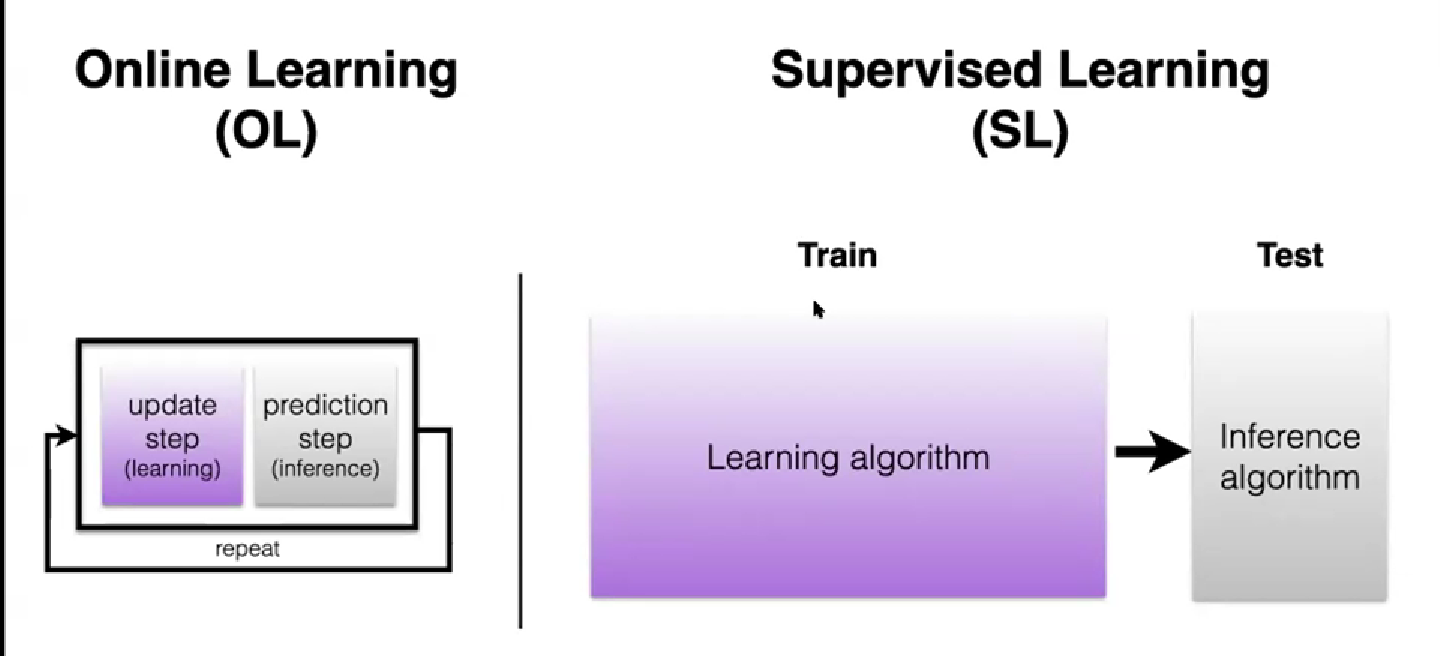
\includegraphics[scale=0.25]{figures/OLSL.png}
\end{center}
\caption{Comparison of Online Learning (OL) with Supervised Learning (SL)}
\label{fig:OLSL}
\end{figure}

In online learning, we have an update step followed by the prediction step. This pair of actions are repeated during the operation of the model. This relationship can be visualized in Fig. \ref{fig:OLSL}.

\begin{figure}[H]
\begin{center}
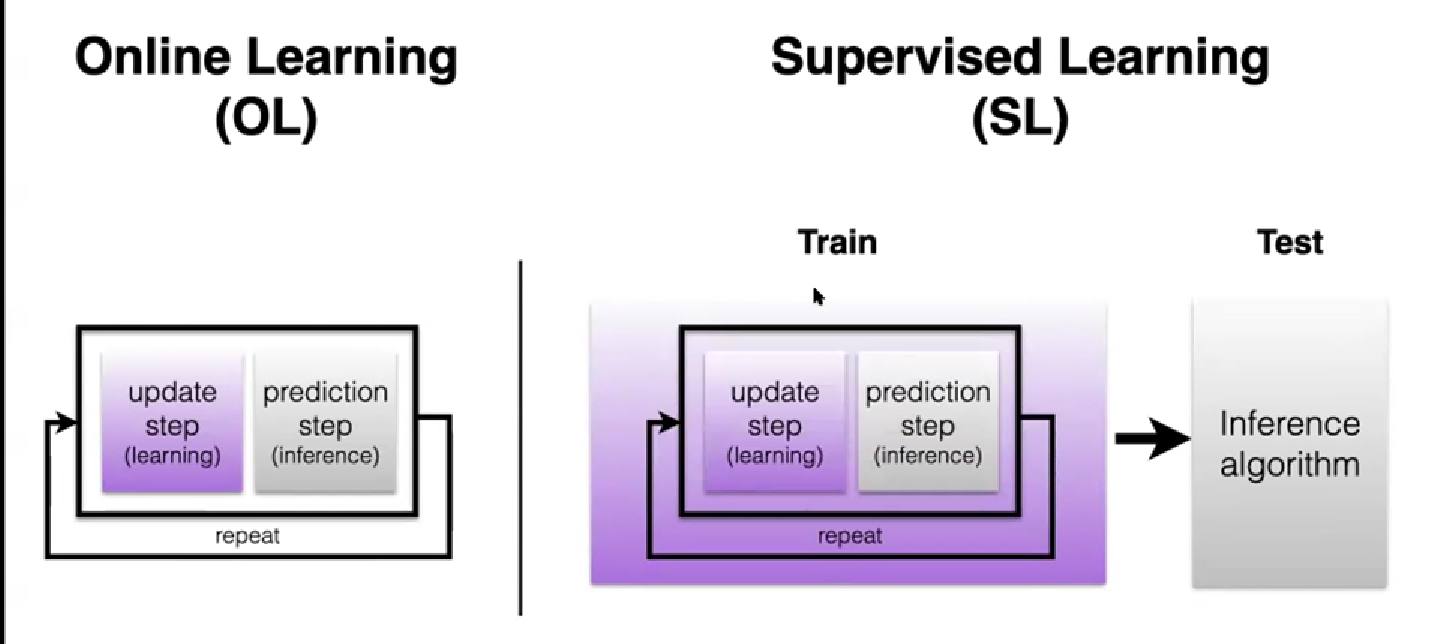
\includegraphics[scale=0.25]{figures/OLinsideSL.png}
\end{center}
\caption{Online Learning can be represented within a Supervised Learning model}
\label{fig:OLinSL}
\end{figure}

Whereas, in supervised learning problems, we train the model with the available data and then utilize the trained algorithm for inference. Often, we can include online learning algorithms within these supervised learning models, as shown in Fig. \ref{fig:OLinSL}.

Therefore, \textbf{most supervised learning algorithms can be solved used online learning models}.

%Length requirement 1-2 pages.
\section{Online Support Vector Maxines}

\subsection{Geometric Intuition}
\subsubsection{Hyperplanes in 2D}

\begin{figure}[h]
    \centering
    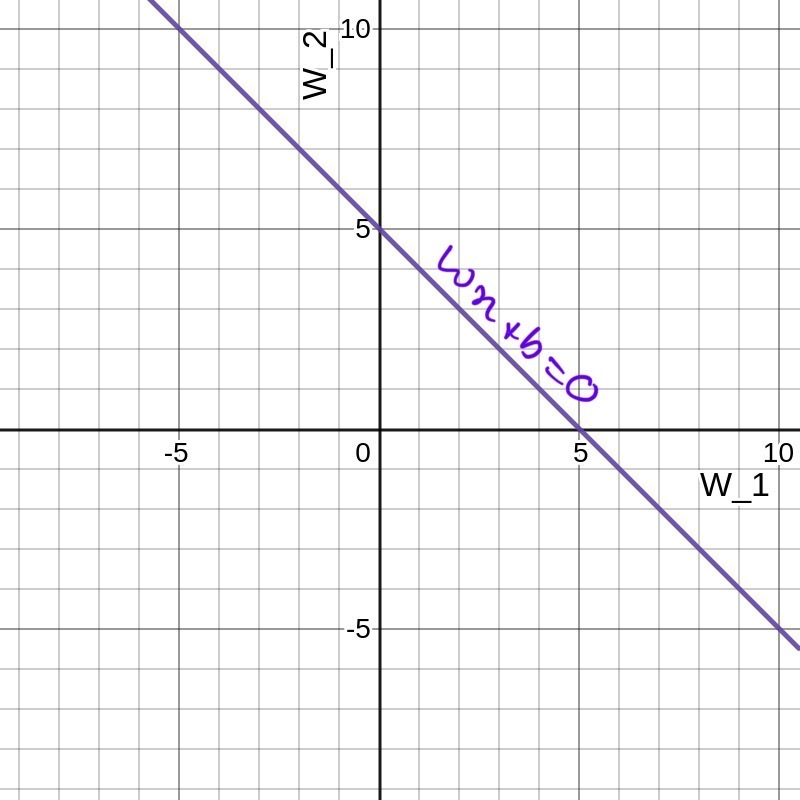
\includegraphics[scale = 0.40]{figures/lineParameterization.jpg}
    \caption{Line parameterization in 2D}
    \label{fig:2DParameterization}
\end{figure}

We can represent hyperplanes in 2D using different parameterizations. One of the parameterizations that we can use is:

\begin{equation} \label{eq:2Dparam}
    w_{1}x_{1} + w_{2}x_{2} + b = 0
\end{equation}

Therefore, to fully represent the line in 2D we need a total of 3 parameters, $w_{1}$, $w_{2}$ and $b$. Here, $w \in R^{2}$

A shorthand for Eq. \ref{eq:2Dparam}, can also be:

\begin{equation} \label{eq:2DParamShort}
    w \cdot x = 0
\end{equation}

Here, in Eq. \ref{eq:2DParamShort}, $w \in R^3$.

An important property of such hyperplanes, is that any normalization can be chosen for $w$, such that the following equation holds:

\begin{equation}\label{eq:lambdaParameterization}
    \lambda (w_1 x_1 + w_2 x_2 + b ) = 0
\end{equation}

This implies that $w$ can be normalized by any scalar value, $\lambda$. Therefore, the line represented in Fig. \ref{fig:2DParameterization}, remains the same, even though $w$ is being normalized by different values.

Using Eq. \ref{eq:2DParamShort}, we can find the perpendicular distance of the line visualized in Fig. \ref{fig:2DParameterization} from the origin through the following steps:

We divide Eq. \ref{eq:2DParamShort} with $||w||$, such that:

\begin{equation}
    \dfrac{w}{||w||} \cdot x + \dfrac{b}{||w||} = 0
\end{equation}

We can rearrange this equation and compare it to the normal form of a line:

\begin{equation}\label{eq:normalFormPre}
    \dfrac{w}{||w||} \cdot x + 0 =  - \dfrac{b}{||w||}
\end{equation}

\begin{equation} \label{eq:normalForm}
    x \cos{\theta} + y \sin{\theta} =  \rho
\end{equation}

Eq. \ref{eq:normalForm}. is equivalent to Eq. \ref{eq:normalFormPre} holds only if $\theta$ is equal to $0^\circ$. This implies that the distance to the origin $\rho$ is equal to $\dfrac{b}{||w||}$.

Consider the now we have another line, offset from the first line that we saw in Fig. \ref{fig:2DParameterization}. We visualize the pair of lines as follows:

\begin{figure}[h]
    \centering
    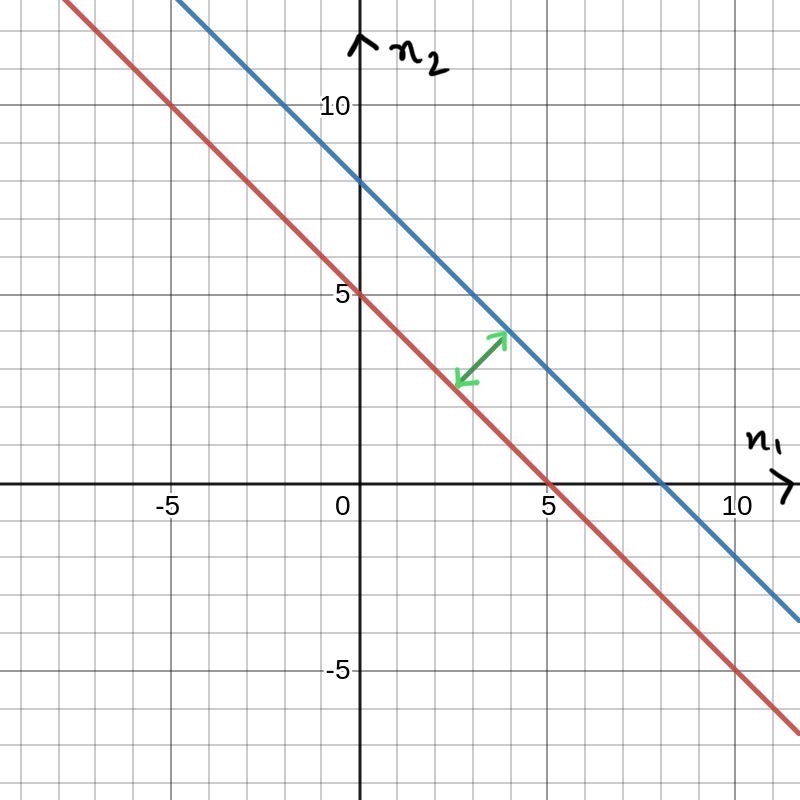
\includegraphics[scale = 0.30]{figures/lineDistance.jpg}
    \caption{A second line parallel to the first line, offset by some distance}
    \label{fig:22DLines}
\end{figure}

We can now find the distance between the pair of lines as follows:

The second line can be described as:
\begin{equation}
    w \cdot + b = - 1
\end{equation}

It's distance from the origin (following the same schema as Eq. \ref{eq:normalFormPre} and Eq. \ref{eq:normalForm}) is given as:
\begin{equation}
    \rho_b = \dfrac{b + 1}{||w||}
\end{equation}

Therefore, the distance between the two lines is:

\begin{equation} \label{eq:dist2lines}
    \rho_{d} = \dfrac{1}{||w||}
\end{equation}

Similarly, for a hyperplane in 3D the only change that we have to make to our equations is the dimensionality of $w$. Instead of being 2-dimensioned in the previous case, $w$ will now be a 3-dimensioned vector.

Consider we have 2 planes in a 3-dimensioned space as shown in Fig. \ref{fig:3DPlanes}:

\begin{figure}[h]
    \centering
    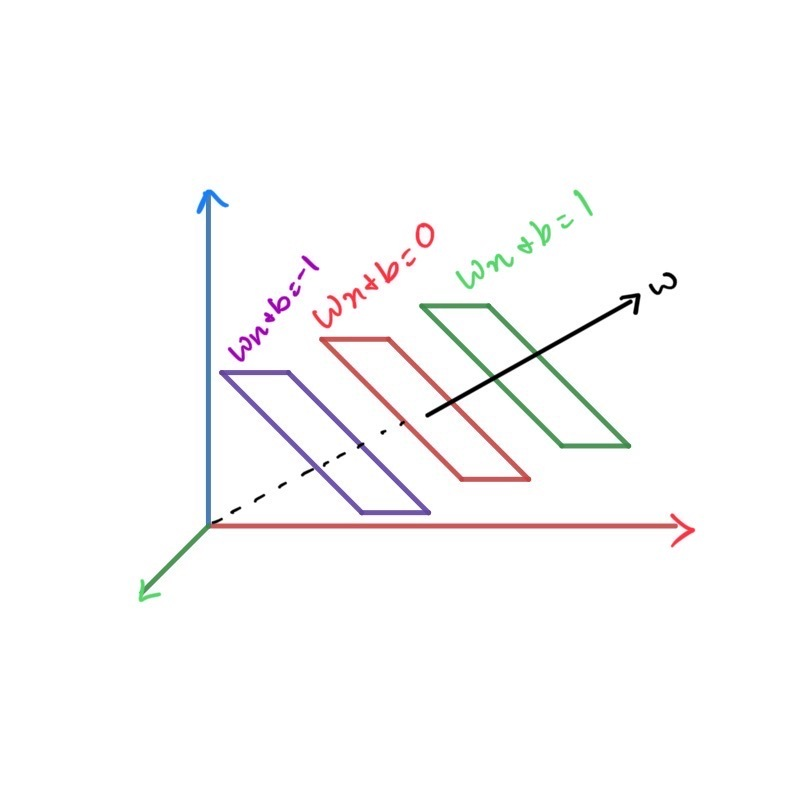
\includegraphics[scale = 0.40]{figures/planeDistance.jpg}
    \caption{Planes in 3D, separated by some distance}
    \label{fig:3DPlanes}
\end{figure}

Since we know the equation of the planes, and their distances to the origin through our previously, derived equations in Eq. \ref{eq:normalForm} and \ref{eq:normalFormPre}, we find the distance between the outermost planes as:

\begin{equation}
    \rho_{OD} = \dfrac{2}{||w||}
\end{equation}


\section{Support Vector Machines (SVM)}
\normalfont

\subsection{Introduction}
Consider the binary classification problem, where we have two clusters of data as shown here:

\begin{figure}[h]
    \centering
    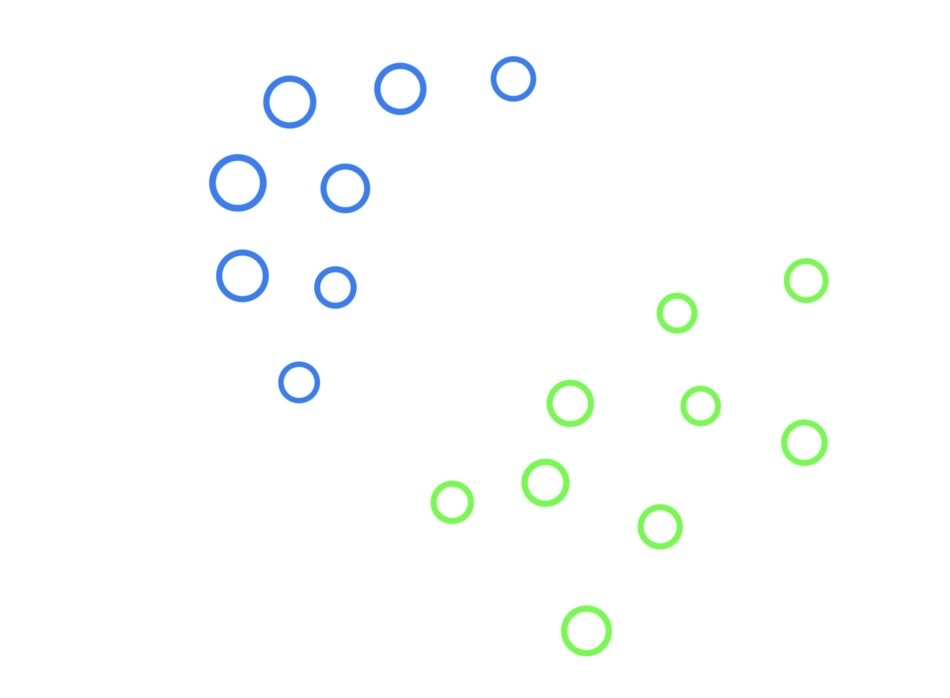
\includegraphics[scale = 0.25]{figures/OGData.jpg}
    \caption{Two clusters of data that have to be separated with a suitable hyperplane $w$}
    \label{fig:DataClusters}
\end{figure}

Our objective is to come up with a hyperplane that best separates this data, such that we have perfect classification between these two classes. Even though we can have any  number of hyperplanes, $w$ that split the data reasonably, intuitively the $w$ that's farthest away from the interior-most points of these two clusters will perfectly classify the data into these two clusters.

Graphically this hypothetical $w$ can be represented as:

\begin{figure}[h]
    \centering
    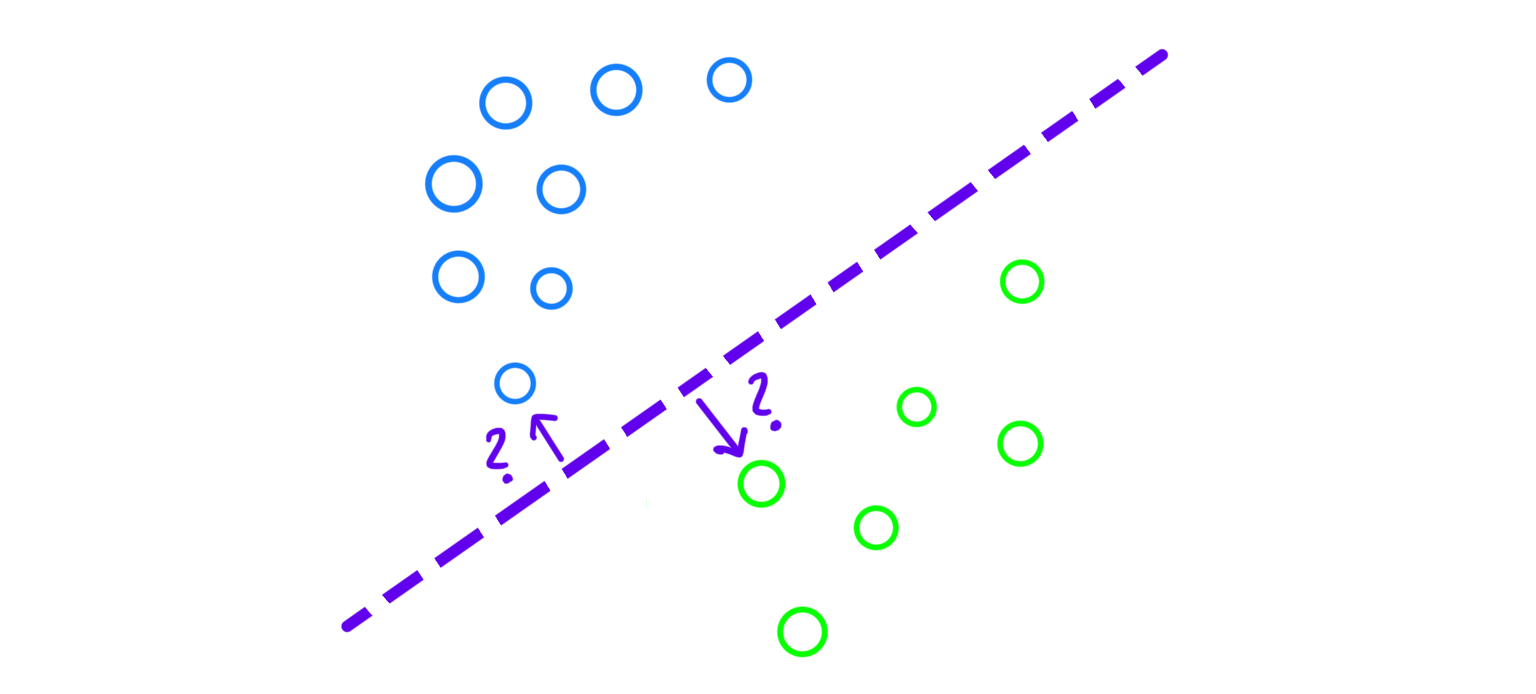
\includegraphics[scale = 0.25]{figures/HowToData.PNG}
    \caption{Hyperplane, $w$, that has the maximum distance from the innermost points of both clusters}
    \label{fig:maxMargin}
\end{figure}

This hyperplane, that has the "maximum margin" to the innermost points, is also the plane, $w$, most likely to be the most stable to perturbations in the data. The innermost points of each cluster that form the definition of the margin to the given hyperplane $w$ are also called "support vectors", and therefore, these planes are also called "Support Vector Machines" or SVMs.

\subsection{Objective of Hyperplanes}

The objective of the SVM is to find a hyperplane, $w$, such that the hyperplanes that define the margin of two clusters is maximised. This objective can be visualized in Fig. \ref{fig:hyperPlaneMargin}:

\begin{figure}[h]
    \centering
    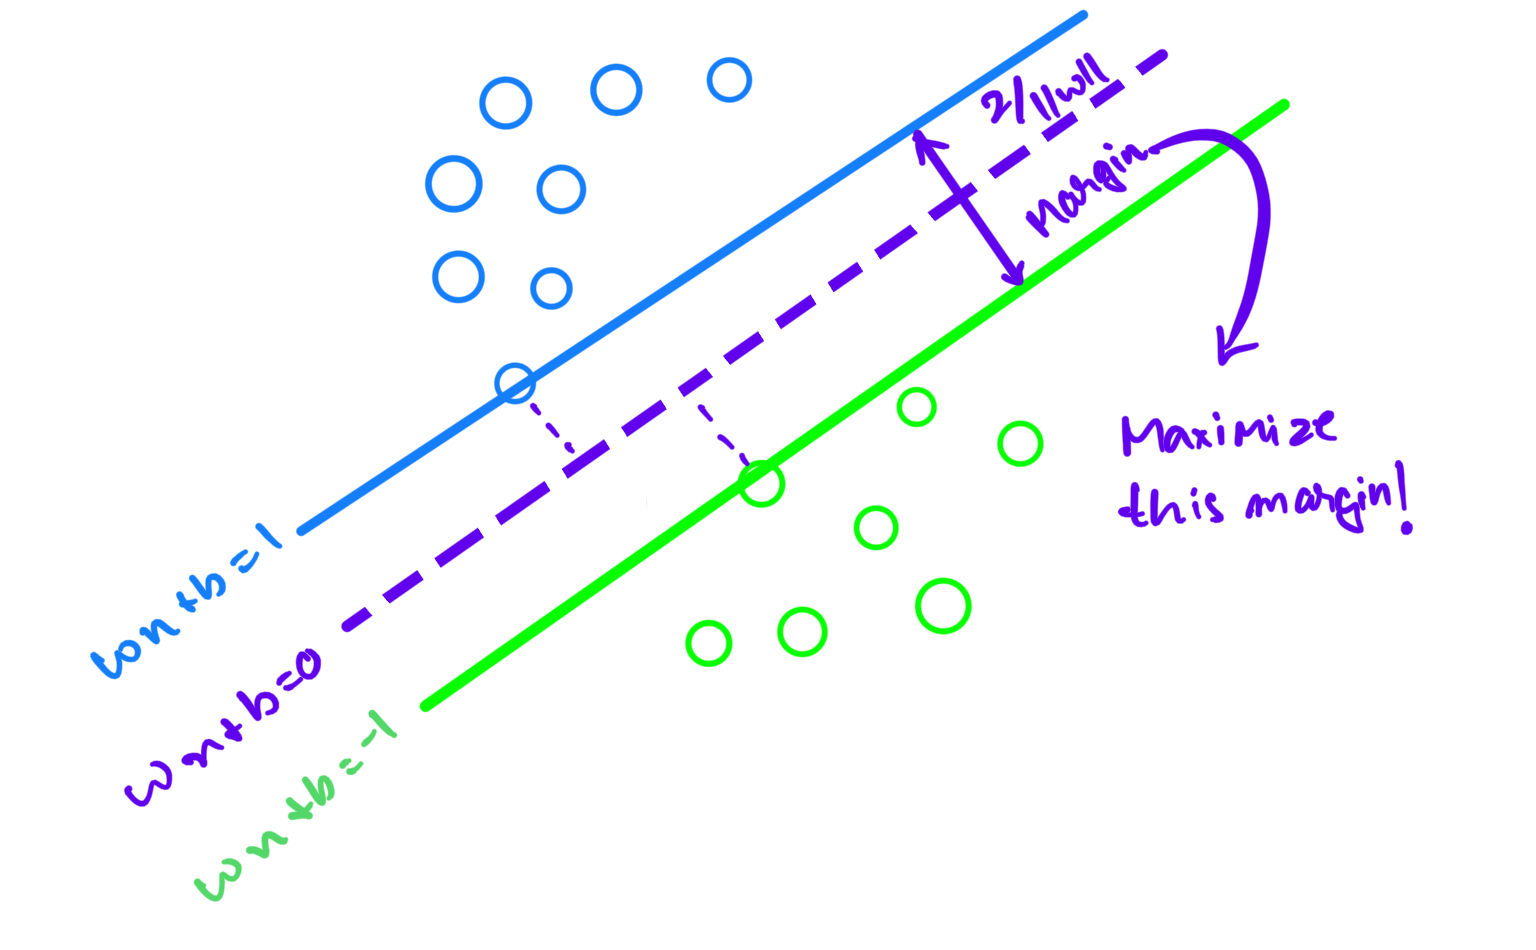
\includegraphics[scale=0.28]{figures/SVMIntro.PNG}
    \caption{The objective of SVM is to find the hyperplane, $w$, such that the margin between the clusters is maximised}
    \label{fig:hyperPlaneMargin}
\end{figure}

From Eq. \ref{eq:dist2lines}, we see that in order to maximise the distance between the two hyperplanes, we have to maximise the term $\dfrac{2}{||w||}$, i.e,

\begin{equation}
    \rho_{max} = \max_{w} \dfrac{2}{||w|||}
\end{equation}

Referencing Fig. \ref{fig:hyperPlaneMargin}, the objective of this SVM is to correctly classify any given data point that it encounters into the correct cluster. 
Let's look at what that would mean mathematically:

\begin{equation}\label{eq:conditionalSVM}
    w \cdot x + b  = 
    \begin{cases}
    +1, & \text{if}\ y_{i} = +1 \\
    -1, & \text{if}\ y_{i} = -1 \forall\ i \in [1, 2, 3 \dots N]
    \end{cases}
\end{equation}

Eq. \ref{eq:conditionalSVM} would imply that the SVM would always correctly label the given $x_{i}$ into one of the clusters. This is the expected performance of the given SVM.

In order to maximize Eq. \ref{eq:conditionalSVM}, we can minimize the following equation instead:

\begin{equation}\label{eq:modifiedConditionalSVM}
    \min_{w} ||w||^{2}
\end{equation}

Given the constraint,

\begin{equation}\label{eq:modifiedConditionalSVMConstrain}
    y_{i}(w \cdot x_{i} + b) \geq 1 \text{, } \forall i \in [1, 2, \dots N]
\end{equation}

In Eq. \ref{eq:modifiedConditionalSVM}, we square $w$ in order to introduce a greater penalty on $w$. The minimum value of $||w||$ will be the same as the minimum value of $||w||^2$, which justifies this substitution. In Eq. \ref{eq:modifiedConditionalSVM}, since we're performing binary classification (i.e, predicting one of two labels $\hat{y}$ in $[-1, 1]$), we can multiply the output of the classification of the SVM with the label, to arrive at the condition within the equation.

Therefore, we can formalize the working of an SVM as:

\textbf{Objective Function}:

\begin{equation}\label{eq:SVMObjective}
    \min_{w} ||w^2||
\end{equation}

\textbf{Constraints}

The objective function in Eq. \ref{eq:SVMObjective} is subject to hard constraints:

\begin{equation}
    y_{i}(w \cdot x_{i} + b) \geq 1 \\
    \text{For i}  \in [1, 2 \dots N]
\end{equation}

This problem is known as a \textbf{Convex Quadratic Problem} (QP) with linear constraints. Such problems might have unique solutions, but may not satisfy the constraints of the data (i.e, the data is not separable or is noisy).

Such SVMs are called \textbf{"Hard SVMs"}, since we make the assumption that all constraints can be satisfied. This may not be the case at all times, as we see below.

% \subsubsection{Mathematical representation of SVM}

% SVM is linear classifier which tries to define a hyperplane such that it maximises the distance between different classes of data. Mathematically speaking, SVM tries to  maximise the value of $\dfrac{2}{||\mathbf{w}||}$, (where $\mathbf{w}$ is set of weights defining the hyperplane) and to maximise the value of $\dfrac{2}{||\mathbf{w}||}$, we can minimise the value of $\mathbf{||w||}$. Since the minimum of $\mathbf{||w||^2}$ and $\mathbf{||w||}$ will be the same, we use the $\mathbf{||w||^2}$ so that there is a higher penalty to $\mathbf{||w||}$ when there is a wrong prediction.

% The objective function here is $\mathbf{min_w||w||^2}$ and is called as the \textbf{Primal Formulation} of a linear SVM

% The hyperplanes can be mathematically defines as:


% $\mathbf{w.x_i+b \geq +1}$ if ${y_i=+1}$ and \\
% $\mathbf{w.x_i+b \leq +1}$ if ${y_i=-1}$
% \\where $\mathbf{y_i}$ represents the true label for an input $\mathbf{x_i}$ 
% \\
% \\The above expressions can be combines to write:
% \\$\mathbf{y_i(w.x_i+b) \geq 1}$ for i=1,...N
% \\This is a convex quadratic programming problem and a unique solution exists for it but it may be possible that the data is not linearly separable.


% Something to note here is that the term on the right side does not necessarily need to be one and can be any scalar value. It is just by convention the value is taken to be 1. If this value is taken more than 1, the distance between the two hyperplanes of two labels shall increase.

% The discussion above is classified as \textbf{Hard SVM}

\subsubsection{Soft SVM}

The above discussion holds true when the data is linearly separable. However, when working with real data, it may not be linearly separable and this is where we use soft margins to separate the data. 

\begin{figure}[H]
\begin{center}
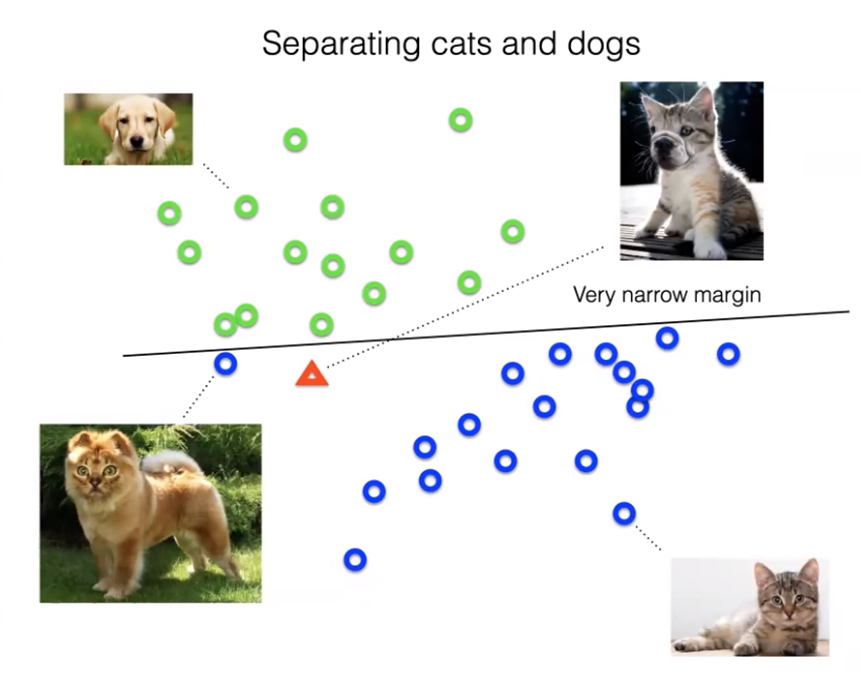
\includegraphics[scale=0.25]{figures/HardSVM.png}
\end{center}
\caption{Performance of Hard SVM of linearly in-separable data}
\label{fig:HardSVMPerf}
\end{figure}

Considering Fig. \ref{fig:HardSVMPerf}, we can see that the data is not linearly separable.  This is because, some of the dogs look slightly like cats and vice versa. As we can see from the data,there is a very small margin between the labels of cats and dogs and in attempts to rightly classify each image, the whole line will be shifted for very rare cases. Therefore, we should allow for some miss-classification if we can get more robust classification by coming up with a hyperplane that has a higher margin, at the cost of some miss-classification. This can be classified as classifying the data 'softly'.

\begin{figure}[H]
\begin{center}
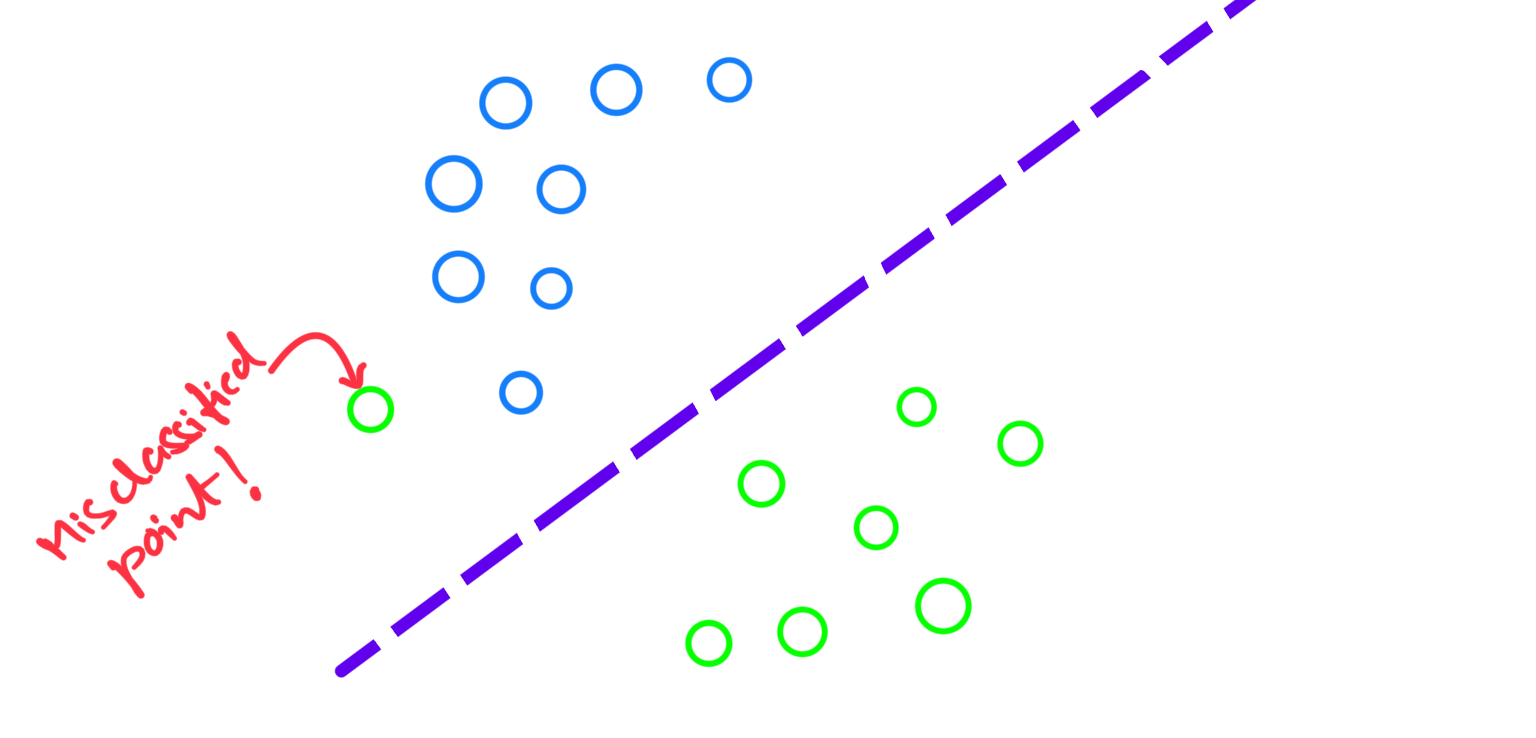
\includegraphics[scale=0.25]{figures/MissClassify.PNG}
\end{center}
\caption{Performance of Soft SVM of linearly in-separable data}
\label{fig:LinearlySeperable}
\end{figure}

Fig. \ref{fig:LinearlySeperable} shows, implementation of some soft SVM at the cost of some miss-classifications. It can be seen that the hyperplane has higher margin and thus, is a better classifier.

\subsubsection{Mathematical interpretation of soft margin}

The 'slack' in classification can be increased by adding a slack variable to the expression we saw earlier for hard SVM classification. Thus, the expression now becomes:

\begin{equation}
y_i(w^T \cdot x_i+b) \geq 1- \xi_i
\end{equation}

Here $\xi$ introduced will decrease the threshold value and some of the values might be miss classified. The value of $\xi$ should ideally be as small as possible because smaller value indicates that the points are on the right side of the hyperplane. The variable $\xi$ is called as the slack variable and geometrically represents the distance of the miss-classified element from the margin. 

\textbf{The object function now becomes}:

\begin{equation}
\min_{w,\xi}||w||^{2} + C \sum{\xi_i}
\end{equation}

\begin{figure}[H]
\begin{center}
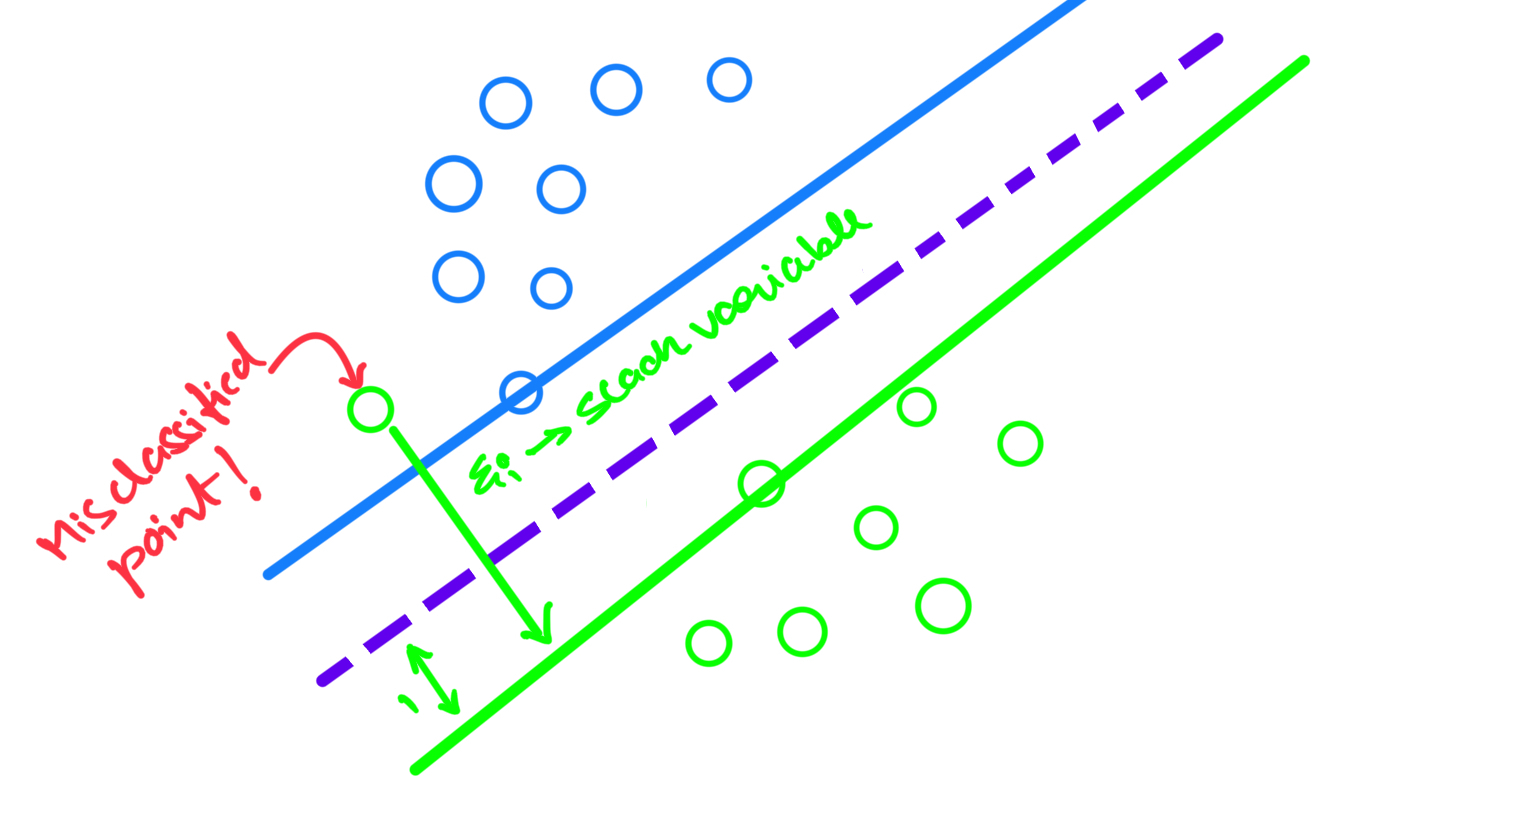
\includegraphics[scale=0.28]{figures/SlackSVM.PNG}
\end{center}
\caption{Geometric interpretation of slack variables in soft SVM}
\label{fig:Slackvariables}
\end{figure}

C here is a regularization parameter. When the value of C is very small, that means that the constraints will be ignored, there will be more miss-classifications and the margins will be higher. And if the value of C is large, constraints won't be ignored, the margin will be small and hence, there will be lesser classifications.


\setlength{\fboxsep}{1.3pt}%
\setlength{\fboxrule}{1pt}%
\begin{figure}[h]
    \centering
    \subfloat{\fbox{{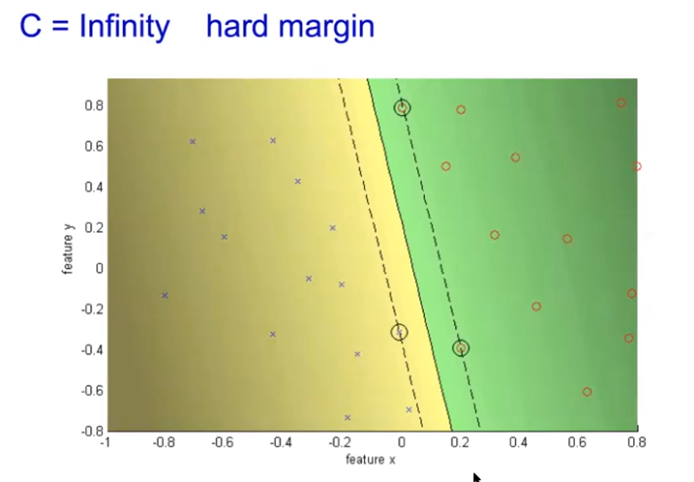
\includegraphics[scale=0.26]{figures/HardMargin.png}}}}%
    \qquad
    \subfloat{\fbox{{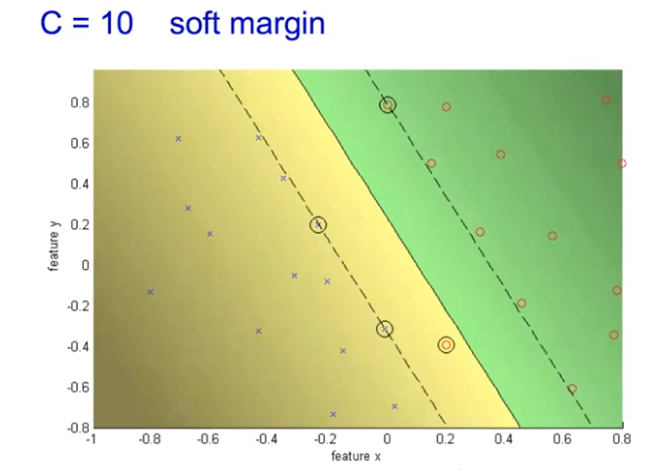
\includegraphics[scale=0.265]{figures/SoftMargin.png}}}}%
    \caption{Comparison between Hard Margin and Soft Margin}%
    \label{fig:SoftMarginsvsHardMargins}%
\end{figure}

\subsubsection{\textbf{Solution for Soft SVM}}

The new objective function $\mathbf{\min_{w, \xi}{||w||^2}+C\sum{\xi_i}}$ when subjected to $\mathbf{y_i(w^{T}x_{i}+b \geq 1-\xi_i)}$ can be solved using Lagrange's method:

Thus, the equation becomes:

\begin{equation}
\min_{w}\dfrac{\lambda}{2}||w||^2+\dfrac{1}{N}\Sigma^N_{i=1}(1-y_i \cdot w^T x_i)
\end{equation}


Where, $\lambda$ is Lagrange's multiplier and $\xi$ becomes:

\begin{equation}
    \xi \geq 1-y_i(w \cdot x_i)
\end{equation}

We can see that when the predictions are correct, the value of $\xi$ can vary from $\infty$ to 1 and when the predictions are wrong, the values can range from 1 to $\infty$. However, we should not be concerned for all the values of $\xi$ but only for those values such that the margins become less or the mistakes are too high. So to bound the value of $\xi$, we use hinge loss such that the new equation becomes:

\begin{equation}
\min_{w}\dfrac{\lambda}{2}||w||^2+\dfrac{1}{N}\Sigma^N_{i=1}\max{(0, 1-y_i w^T \cdot x_i)}
\end{equation}

One thing to note here is that the function is convex here but is not differentiable throughout because of the hinge. Therefore, to solve this function, we introduce sub-gradients. The necessity to introduce sub-gradient arises when a function is not differentiable throughout its input values. In the second sub-figure of \ref{fig:GradientVsSubGradient}, the various lines lower bounding the convex function at the hinge are called the sub-gradients. 

\begin{figure}[H]
\begin{center}
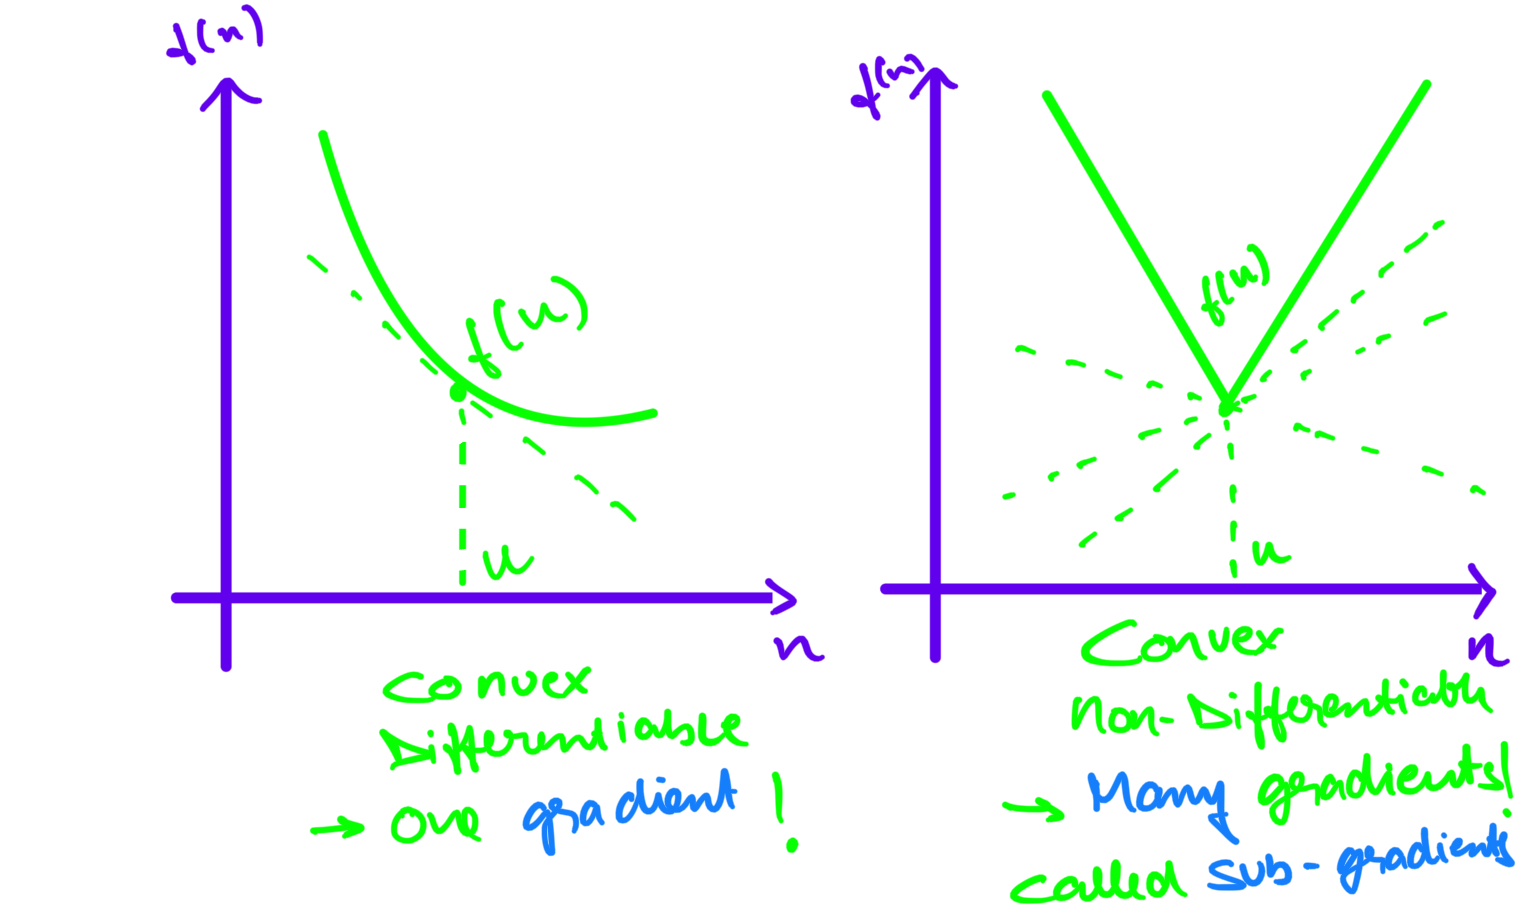
\includegraphics[scale=0.25]{figures/diffNonDiff.PNG}
\end{center}
\caption{Gradient vs Sub-Gradient}
\label{fig:GradientVsSubGradient}
\end{figure}

From all the possible sub-gradients, we can define two gradients for the function such that it can be differentiated:

\begin{equation}
    z_{[m]} = 
    \begin{cases}
    0 & \text{if, }\ y_m w^T x_m \geq 1\\
    -y_{m}x_{m} & \text{otherwise} 
    \end{cases}
\end{equation}

So the algorithm becomes:
% \\1: function SOFTSVM$(\lambda)$
% \\2: $\mathbf{}{\theta^{(0)}=0}$
% \\3: for t=1,...T do
% \\4: \hspace{1cm} $y_d,x_d ~ D$
% \\5: \hspace{1cm}$\theta^{t}=\theta^{t-1}+ y_d.x_d.1[y_d(w^(t).x_d)<1]$
% \\6: \hspace{1cm}$w^{t+1}=\dfrac{1}{\lambda(t+1)}.\theta^{t}$


\begin{algorithm}[H]
\caption{Soft SVM}
\label{algo:SoftSVM}
\begin{algorithmic}[1]
\STATE $\theta^{(0)}=0$ \hfill
\FOR{$t=1,\;\cdots,\;T$}
\STATE $y_d,x_d \sim  D$ \hfill 
\STATE $\theta^{t}=\theta^{t-1}+ y_{d}x_{d} \cdot 1[y_d(w^{t}x_{d})<1]$ \hfill 
\STATE $\hat{y}^{(t)} = h(\textbf{x}^{(t)})$ \hfill 
\STATE $w^{t+1} \leftarrow \dfrac{1}{\lambda(t+1)} \cdot \theta^{t}$ \hfill
\ENDFOR
\end{algorithmic}
\end{algorithm}

In line 5, $y_{d}x_{d}$ is the sub-gradient and the indicator function is the hinge condition, such that the $\theta^{t}$ will only be updated if there is a wrong prediction or if the label is on the wrong side of the hyperplane.

This algorithm is very close to online perceptron algorithm. However something to note here is that in online perceptron algorithm, indicator function is $1\cdot[y_d(w^(t).x_d)<0]$ implying that the perceptron algorithm considers if the prediction is right or wrong and does not consider correctness or in-correctness of the prediction. SVM on the other hand, considers both correctness and the in-correctness of predictions.

\section{Conclusion}

In this lecture, we looked at the underlying mechanics of how Support Vector Maxines work (SVMs). We also learnt the differences between Hard and Soft SVMs, and their performance when presented with linearly separable and in-separable data. We also looked at the need for sub-gradients when dealing with convex, but non-differentiable functions.

\textbf{Note}: We referred to the previous years' scribe notes while preparing this document \cite{Paritosh2021}.

\section{Appendix}


%\section*{References}
%Include your references here. Please cite any resources you found useful.	
%Populate the refs.bib file or list your references manually. Be consistent in formatting!
{
\bibliography{refs}
\bibliographystyle{abbrv}
}

%\section{Appendix}
%This section provides any relevant background material that was not covered in the lectures, but was found to be useful for understanding the material. 
%For example, derivations, theory underlying techniques employed, etc. 

%Additionally, this section can summarizes applications or extensions of these techniques found in the literature. 

\end{document} % Done!